\documentclass[12pt]{standalone}

%% for compilation with htlatex (to produce svg image),
%% uncomment the line below:
%\def\pgfsysdriver{pgfsys-tex4ht.def}

\usepackage{tikz}

\tikzstyle{tensor}=[rectangle,draw=blue!50,fill=blue!20,thick]
\tikzstyle{dots}=[thick]

\begin{document}

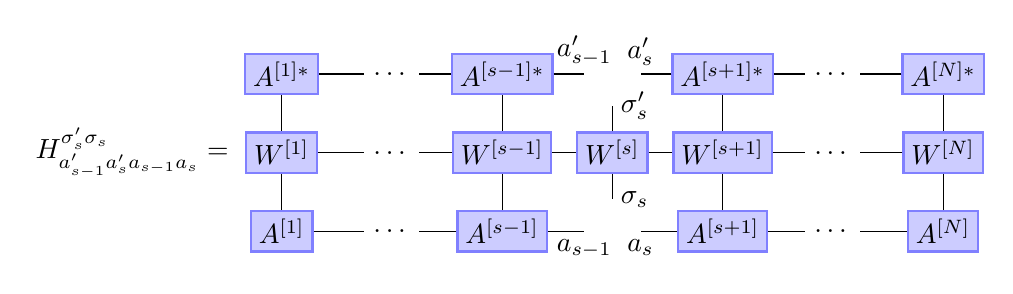
\begin{tikzpicture}[inner sep=1mm]
  \def\sep{1.4};
  %\def\x{1068}

  \foreach \pos/\label in {1/1,3/s-1,5/s+1,7/N} {
    \node[tensor] (\pos \space spin conjugate) at (\pos*\sep, 1.) {$A^{[\label]*}$};
    \node[tensor] (\pos\space spin) at (\pos*\sep, -1.) {$A^{[\label]}$};
    \node[tensor] (\pos) at (\pos*\sep, 0) {$W^{[\label]}$};
    \draw[-] (\pos\space spin conjugate) -- (\pos);
    \draw[-] (\pos) -- (\pos \space spin);
  } 
  
  \node[tensor] (4) at (4*\sep, 0) {$W^{[s]}$};

  \foreach \pos in {2,6} {
    \pgfmathtruncatemacro{\posplusone}{\pos + 1};
    \pgfmathtruncatemacro{\posminusone}{\pos - 1};

    \node[dots] (\pos \space spin conjugate) at (\pos*\sep, 1.) {\dots};
    \node[dots] (\pos \space spin) at (\pos*\sep, -1.) {\dots};
    \node[dots] (\pos) at (\pos*\sep, 0.) {\dots};

    \foreach \name in { , \space spin, \space spin conjugate} {
      \draw (\posminusone \name) to ({\pos \name}.west);
      \draw (\posplusone \name) to ({\pos \name}.east);
    }
  }

  \draw[-] (3) -- (4);
  \node[minimum width=0.7cm, minimum height=0.8cm] (4 spin) at (4*\sep,-1.) {};
  \node[minimum width=0.7cm, minimum height=0.8cm] (4 spin conjugate) at
  (4*\sep,1.) {};
  \draw[-] (3 spin) -- ({4 spin}.west) 
    node[below] {$a_{s-1}$};
  \draw[-] (3 spin conjugate) -- ({4 spin conjugate}.west) 
    node[above] {$a_{s-1}'$};
  \draw[-] (4) -- ({4 spin}.north) node[right] {$\sigma_s$};
  \draw[-] (4) -- ({4 spin conjugate}.south) node[right] {$\sigma_s'$};
  \draw[-] (4) -- (5);
  \draw[-] (5 spin) -- (4 spin.east) 
    node[below] {$a_s$};
  \draw[-] (5 spin conjugate) -- (4 spin conjugate.east) 
    node[above] {$a_s'$};

  \node at (-.5, 0.) {$H_{a_{s-1}'a_s' a_{s-1}a_s}^{\sigma_s' \sigma_s} = $};
    %\draw[-] (1.west) .. controls +(-1.5, 1) and +(1.5, 1) .. (5.east);
\end{tikzpicture}

\end{document}

